\documentclass{jfm-like}
\usepackage{graphicx}
\usepackage{epstopdf, epsfig}

%-------------------------------------------
% additional packages added by KW
%-------------------------------------------
\usepackage{mathrsfs} 
\usepackage{amssymb}
\usepackage{amsmath}
\usepackage{bm}
%-------------------------------------------

\shorttitle{open boundary pressure projection}
\shortauthor{K. B. Winters}

\title{Healing discontinuous derivatives with low-order Bernoulli polynomials}

\author{Kraig Winters
  }

\affiliation{Scripps Institution of Oceanography, University of California San Diego,
La Jolla, CA 92093, USA
}

\begin{document}

\maketitle

% single-paragraph abstract <= 250 words, provides a summary of the main aims and results.
\begin{abstract}
This note documents  a preprocessing procedure for rendering functions $f(x)$ defined on the closed interval $x \in [0,L]$ computationally differentiable using cosine transforms.
The procedure relies on the construction of two low order expansions using Bernoulli polynomials to remove the singularities associated with discontinuous derivatives at $x=0$
and $x=L$ when $f$ is even-extended into $[0,2L]$. These series are easy to construct and can be differentiated semi-analytically given the expansion coefficients. Subtracting
these series from $f$ leaves behind a smooth, $Q$-times differentiable function $f_Q(x)$ where $(Q+1)/2$ is the number of terms used in the series expansions.
\end{abstract}

%\begin{keywords}
%Authors should not enter keywords on the manuscript, as these must be chosen by the author during the online submission process and will then be added during the typesetting process (see http://journals.cambridge.org/data/\linebreak[3]relatedlink/jfm-\linebreak[3]keywords.pdf for the full list)
%\end{keywords}

\section{The problem}
For functions $f(x)$ defined in the closed interval $x \in [0,1]$, the even extension of $f$ into the domain $[0,2L)$ is, by construction, a continuous $2L$ periodic  function with
discontinuous derivatives at $x=0$ and $x=L$. Nevertheless, $f(x)$ has an N-mode cosine series expansion that matches the function values at the N equally spaced grid points in $[0,L]$. Cosine transforms
allow for efficient construction of anti-derivatives using the well-known procedure of multiplication by inverse wavenumbers in the Fourier domain followed by an inverse cosine transform.
This is very useful, for example, when solving the Poisson equation $ \phi_{xx} = f(x)$ subject to homogeneous Neumann conditions $f_x=0$ at $x=0,L$.

The problem, however, is that the cosine transform of $f(x)$ cannot be simply differentiated by the usual transform, wavenumber multiplication and inverse transform procedure owing to the discontinuities
in the derivative associated with the even extension to $x \in [0,2L)$. For the generalized boundary-forced version of {\bf flow\_solve}, the algorithm is fundamentally dependent on a fast cosine transform
treatment of the Poisson equation for pressure. Since the dependent variables satisfy no particular symmetries, direct differentiation using fast cosine transforms leads to unacceptable Gibbs oscillations in the
computed derivatives. Our objective here is to remove the Gibbs phenomena while retaining the accuracy and efficiency of fast cosine transforms.

\section{The Bernoulli polynomial approach}
Let the even extension of $f(x)$ be decomposed as follows (c.f. Eckhoff, 1998, Lanczos, 1966).
\begin{equation}
f(x) = f_Q(x) + \sum_{n=1, {\rm odd}}^Q A_n \, U_n(x) + + \sum_{n=1, {\rm odd}}^Q B_n \, U_n(x-L) ~~~,~~~ x \in [0,2L)
\label{f_expansion}
\end{equation}
where $Q$ is a relatively small integer. The functions $f(x)$ and $U_n(x)$ are $2L$ periodic and $U_n$ is related to the Bernoulli polynomial of degree $n+1$ as follows:
\begin{equation}
U_n(x) = - \frac{(2L)^n}{(n+1)!} \, B_{n+1} \left( \frac{x}{2L} \right).
\end{equation}
The two series are based on expansions of the even Bernoulli polynomials about the two singular points $0$ and $L$ of the even function $f$. Odd order Bernoulli polynomials are excluded due to symmetry
and $B_1(x)$ is unnecessary because the function $f$ itself is continuous at the singular points. The series expansions are designed to match the continuity properties of $f$. For simplicity of notation, the two
series in Eq. (\ref{f_expansion}) are denoted $S_0(x)$ and $S_L(x)$ so that
\begin{equation}
f(x) = f_Q(x) + S_0(x) + S_L(x).
\end{equation}

The two series have useful properties for our purposes here. First, the Bernoulli polynomials themselves can be differentiated semi-analytically, i.e. in terms of Bernoulli function evaluations:
\begin{equation}
\frac{\rm d}{ {\rm d} x} B_n(x) = n \, B_{n-1}(x).
\end{equation}
Second, $U_1(x)$ ,and thus $S_0(x)$, has a discontinuous derivative at the left singular point $x=0$ but is even symmetric, i.e. has zero derivative at the singular point $x=L$. Similarly, $U_1(x-L)$ and $S_L(x)$
have discontinuous derivatives at $x=L$ but zero derivatives at $x=0$. These properties are inherited from the behavior of $B_2(x)$, the lowest order polynomial in the expansions. All higher order terms in the expansions
are multiples of the even Bernoulli polynomials and thus have zero derivatives at both singular points $0$ and $L$.

\section{Computing the expansion coefficients}
Given the properties of the two expansions $S_0$ and $S_L$ it is straightforward to design constraints to determine the coefficients $\{A_n\}$ and $\{B_n\}$. Ideally, $S_0$ should match the singular behavior of
$f(x)$ near $x=0$ while being well-behaved in the interior of the domain with a vanishing derivative at $x=L$. Similarly, $S_L$ should absorb the singular behavior near $x=L$. There are $M = (Q+1)/2$ terms in each series.
For the $N$  points $x_i$ in $[0,L]$, the constraints are simply
\vspace{12pt}
\begin{itemize}
\item $S_0(x_i) = f(x_i) ~~~i=j,j+1, \dots M-1$, ~~(j=0)
\item $S_L(x_i) = f(x_i) ~~~i=j,j+1, \dots N-1$, ~~(j=N-M)
\end{itemize}
\vspace{12pt}

\noindent {\em i.e.} that the two series match the function $f(x)$ at the M points nearest the singularities. These represent small linear systems for the expansion coefficients and
can be written in matrix form as follows:

\footnotesize
\begin{equation}
\begin{bmatrix}
U_1(x_0) & U_3(x_0) & U_5(x_0) & \dots & U_Q(x_0) \\
U_1(x_1) & U_3(x_1) & U_5(x_1) & \dots & U_Q(x_1) \\
\dots  & \dots  & \dots  & \dots & \dots  \\
U_1(x_{M-1}) & U_3(x_{M-1}) & U_5(x_{M-1}) & \dots & U_Q(x_{M-1})
\end{bmatrix}
\begin{bmatrix}
A_1 \\ A_3 \\ \dots \\ A_{Q} 
\end{bmatrix}
=
\begin{bmatrix}
f(x_0) \\ f(x_1) \\ \dots \\ f(x_{M-1})
\end{bmatrix}
\label{eq:mat1}
\end{equation}
\normalsize

\vspace{12pt}
and, for $j=N-M$,
\vspace{12pt}

\footnotesize
\begin{equation}
\begin{bmatrix}
U_1(x_{j}-L) & U_3(x_{j}-L) & U_5(x_{j}-L) & \dots & U_Q(x_{j}-L) \\
U_1(x_{j+1}-L) & U_3(x_{j+1}-L) & U_5(x_{j+1}-L) & \dots & U_Q(x_{j+1}-L)\\
\dots  & \dots  & \dots  & \dots & \dots  \\
U_1(x_{N-1}-L) & U_3(x_{N-1}-L) & U_5(x_{N-1}-L) & \dots & U_Q(x_{N-1}-L)
\end{bmatrix}
\begin{bmatrix}
B_1 \\ B_3 \\ \dots \\ B_{Q} 
\end{bmatrix}
=
\begin{bmatrix}
f(x_{j}) \\ f(x_{j+1}) \\ \dots \\ f(x_{N-1})
\end{bmatrix}
\label{eq:mat2}
\end{equation}
\normalsize


For $Q=7$ these are $4 \times 4$ linear systems. Constructing the matrices involves evaluations of relatively low even order Bernoulli polynomials at a small set of grid points.
The coefficient matrices are independent of the values of $f$ and so can be constructed and decomposed once into $LU$  factors and then used
for many different data vectors $f(x_i)$. 


\section{An illustrative example}
To illustrate the approach we consider an explicit example. Let the number of grid points $N=257$ and the domain length $L=1$. Let
\begin{equation}
f(x) = e^{\alpha x} ~~~{\rm with}~~~ \alpha = 3/2
\end{equation}
and take Q=7.

Figure \ref{fig:decomposition} (a) shows the function $f(x)$ evaluated at N discrete points in $[0,L]$. The function is not periodic over this domain, nor do its derivatives vanish
at the end points. Consequently, the $2L$ periodic even extension of $f(x)$, shown in panel (b), has discontinuous derivatives at $x=0$ and $x=L$. Equations (\ref{eq:mat1})
and (\ref{eq:mat2}) were solved for the expansion coefficients $A_n$ and $B_n$ and these were used to construct the two series $S_0(x)$ and $S_L(x)$, shown separately
in (a). $S_0(x)$ matches the function $f$ near $x=0$ and has zero derivative near $x=L$. Conversely,  $S_L(x)$ matches the function $f$ near $x=L$ and has zero derivative near $x=0$.
The sum of these two series is shown in (b), even extended to $x \in [0,2L]$. It has discontinuous derivatives at $x=0$ and $x=L$ corresponding to those in $f$. Subtracting these two series
from $f(x)$ leaves the function $f_Q(x)$ shown in red. This function is $2L$ periodic and has continuous derivatives everywhere, rendering it suitable for standard Fourier differentiation
in $[0,2L)$ or via cosine transforms in $[0,L]$.
 \begin{figure}
  \centerline{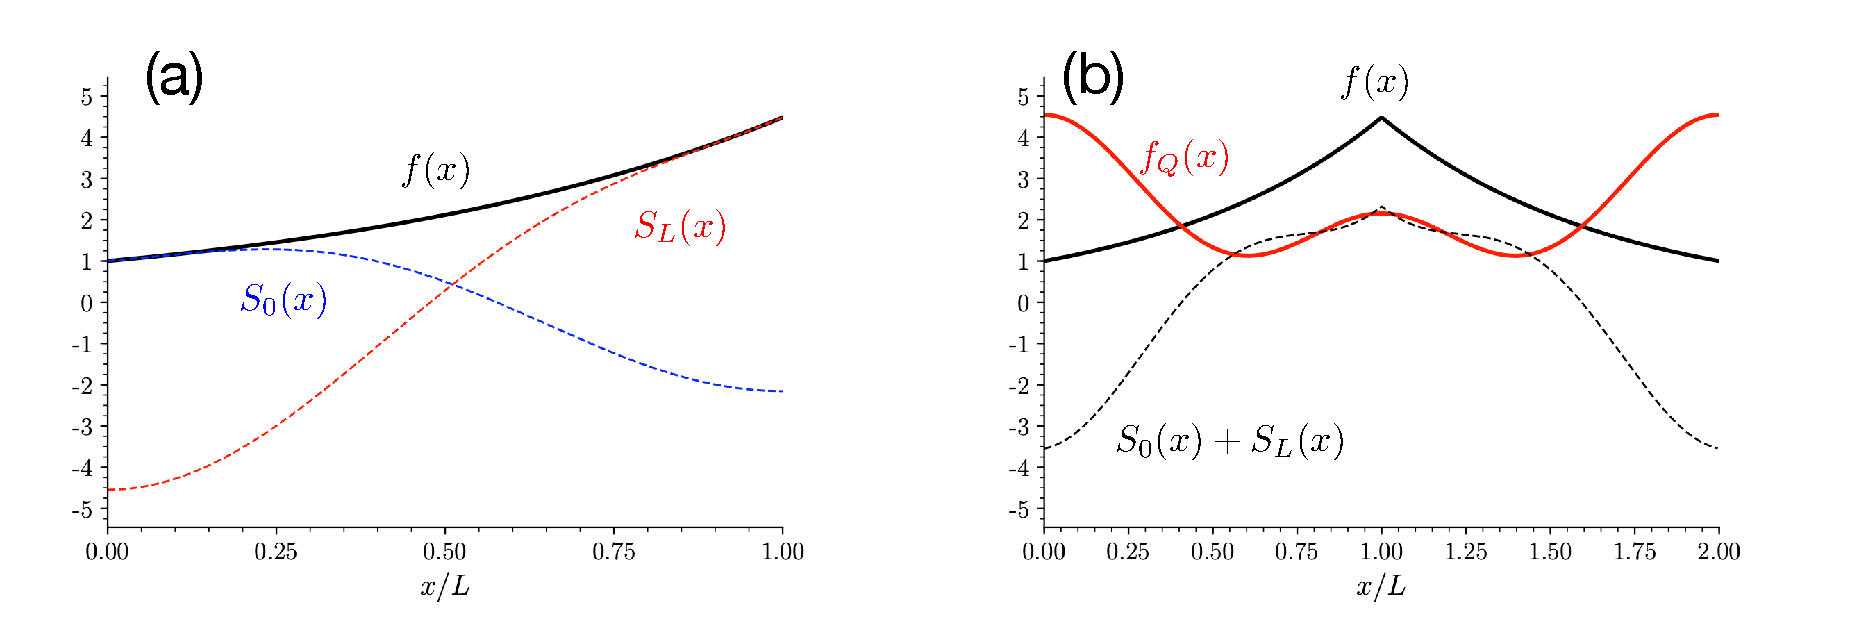
\includegraphics[width=1.0\textwidth]{FIGS/exp_figs/decomposition.eps}}
  \caption{Explicit example for $f(x)=e^{\alpha x}$ using 4 term series expansions with Q=7. (a) The function $f$ and the two series expansions  $S_0$ and $S_L$ shown separately.
  (b) The function $f$, $S_0 + S_L$ and $f_Q$, all even-extended to $x \in [0,2L)$.} 
  \label{fig:decomposition}
\end{figure}

Figure \ref{fig:derivs}(a) shows two estimates of $f'(x)$ along with the exact values (black). The first estimate (blue) is obtained by simply ignoring the discontinuity associated with even extending $f$
and multiplying the cosine expansion coefficients by $k$ and inverse transforming. This estimate suffers from Gibbs oscillations near the end points as expected. 
The Bernoulli/cosine estimate is  obtained by differentiating the two series expansions semi-analytically using (2.2) and (2.4) and applying the standard cosine transform differentiation method to 
 $f_Q(x)$. The result is shown in red but is almost completely obscured by the exact values shown in black.  The magnitude of the error in the Bernoulli/cosine estimate, normalized by the maximum magnitude of $f'(x)$,
  is also shown.
 Figure \ref{fig:derivs} (b) Fourier spectra for $f(x)$ and $f_Q(x)$ (both even-extended). This is identical to the corresponding cosine spectra for the functions evaluated in $[0,L]$. The spectrum of $f_Q$ decays rapidly for large $k$ while the spectrum of $f$ is almost flat near $k_{\rm max}$.
 \begin{figure}
  \centerline{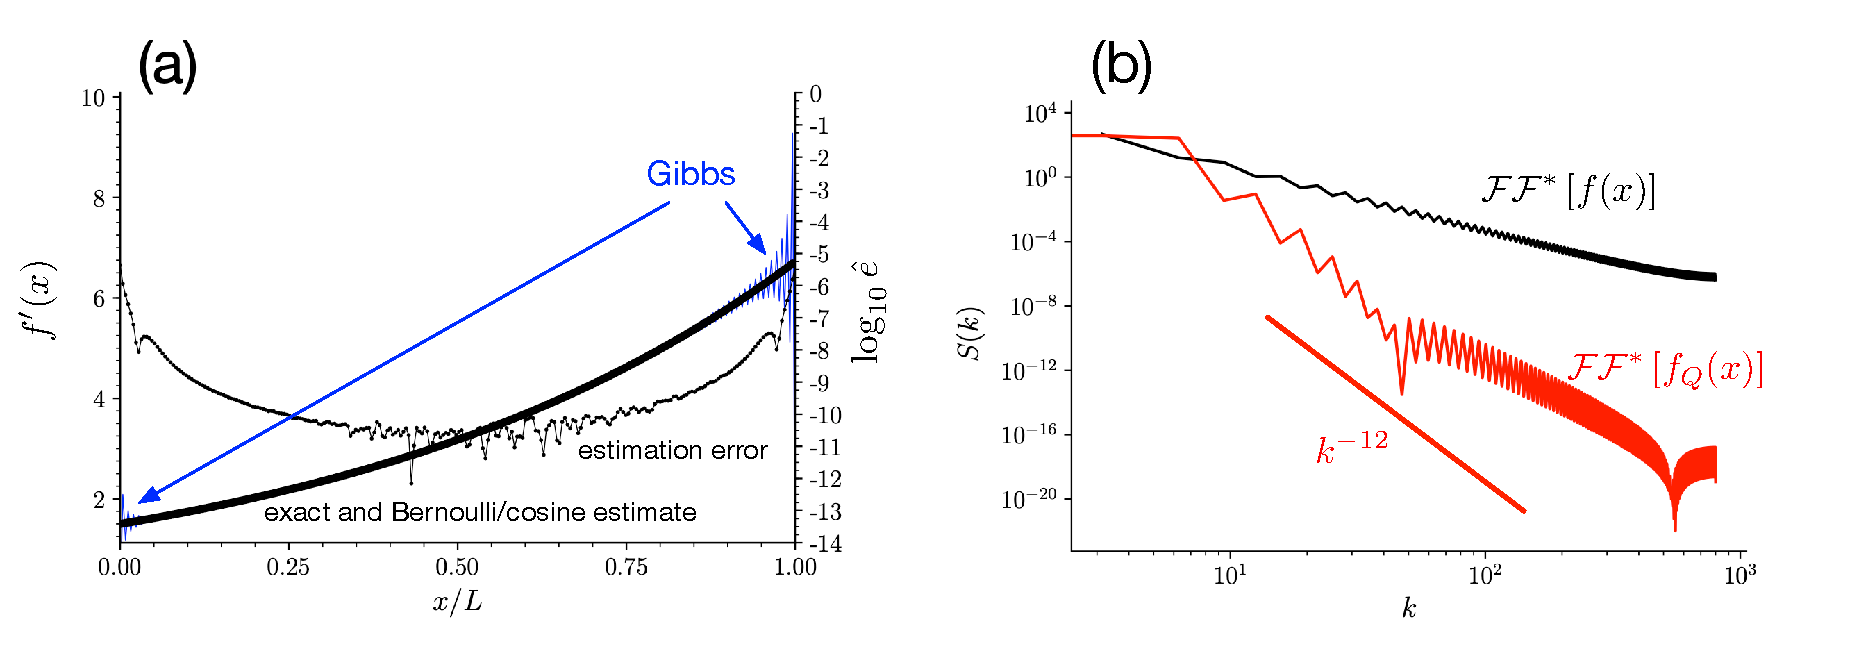
\includegraphics[width=1.0\textwidth]{FIGS/exp_figs/derivs.eps}}
  \caption{Explicit example for $f(x)=e^{\alpha x}$ using 4 term series expansions with Q=7. (a) Estimates of $f'(x)$ and the error in the Bernoulli/cosine approach. (b) Fourier spectra
  of $f(x)$ and $f_Q(x)$.} 
  \label{fig:derivs}
\end{figure}


\section{Misc.}
\subsection{Phase shifted trigonometric functions}
For wave propagation problems, large-scale waves will be passing through a nested subdomain with a time-evolving phase and so we will need to differentiate trigonometric signals with arbitrary phase shifts. An example is
shown in Figure \ref{fig:trig}. Unless the phase shift is $\pm \pi/2$, the even extension of $f$ will have discontinuous derivatives at $x=0,L$.
 \begin{figure}
  \centerline{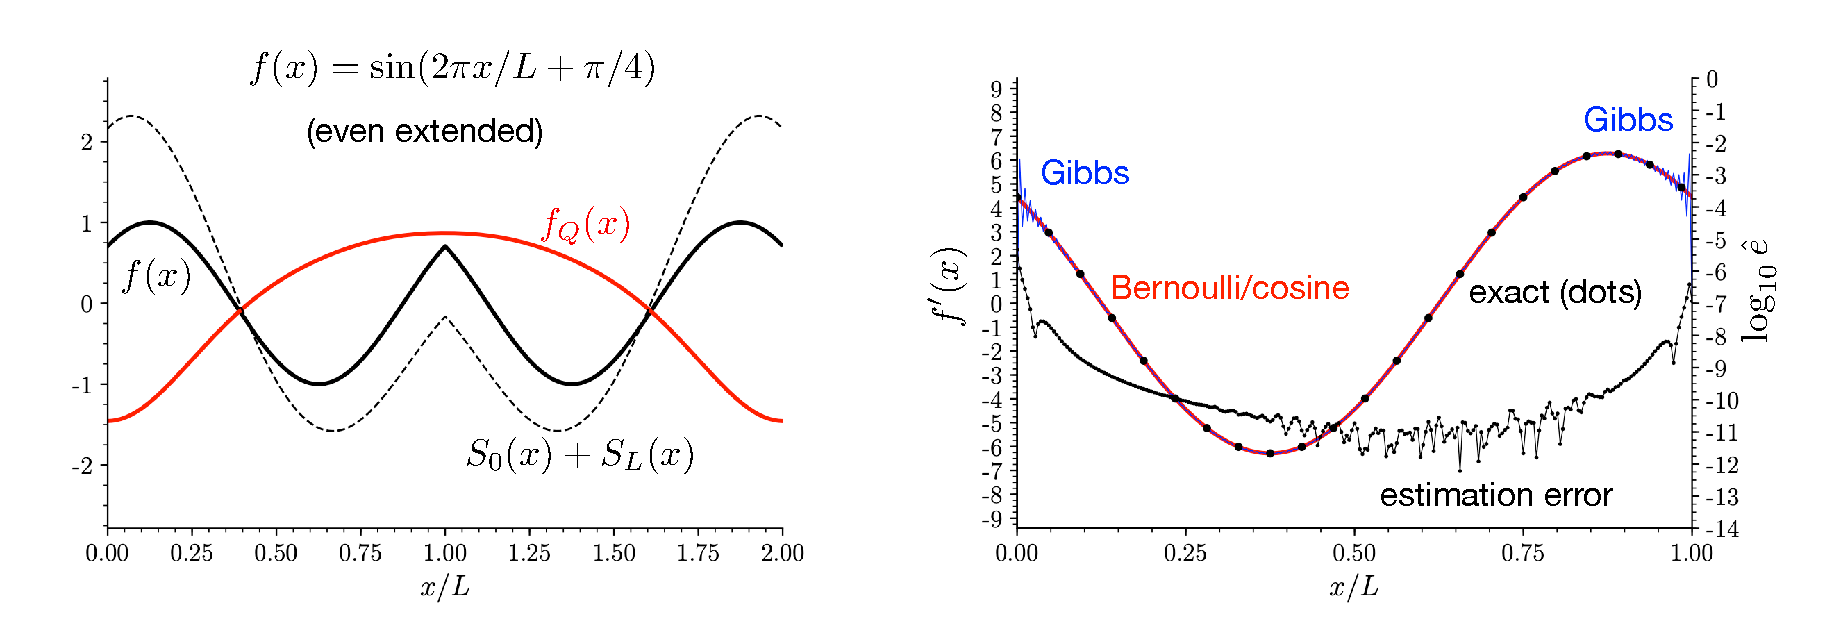
\includegraphics[width=1.0\textwidth]{FIGS/trig_figs/trig_fig.eps}}
  \caption{Explicit example for $f(x)=\sin(2\pi x/L + \pi/4)$ using 4 term series expansions with Q=7. (a) The function $f(x)$, the series $S_0(x)+S_L(x)$ and the easily differentiable difference $f_Q(x)$.}
   \label{fig:trig}
\end{figure}

\subsection{Signals with sharp interior features}
We now consider the case where the magnitude of the derivatives near the end points $x=0,L$ are small in comparison to the derivatives encountered in the interior. This situation might be expected in nested-domain
simulations where the function values specified at the boundaries were computed at much lower resolution and, in the context of a much finer resolution nested domain, vary quite smoothly. By design, we may allow
the flow to develop much finer structures in the interior. This would be especially true if near-boundary sponge layers are used to damp outgoing signals. In this case, we might wonder whether the slightly larger errors
in the near-boundary derivative estimates are worrisome or not. 

To examine this, consider a variant of the first test problem. Let
\begin{equation}
f(x) = e^{\alpha x} + A e^{[(x-x_0)/\gamma]^2} 
\end{equation}
where  $\alpha=3/2$, $A=1$, $\gamma=10^{-2}$  and $x_0=0.425$. Note that $1/\gamma$ is O($N$), where $N=257$ is the number of grid points in $[0,L]$. Thus, the additional interior feature is moderately ``sharp"
for the given resolution while its amplitude is about a third of the difference $(f(L)-f(0)$. The function is intended to be an example of a field that varies smoothly at large scale across a subdomain, a characteristic giving rise
to problematic behavior at the boundaries, that also exhibits numerically challenging small-scale features in the interior.

Figure \ref{fig:bump} shows plots similar to the earlier ones for this example. The true maximum derivative associated with the bump is much larger than the derivatives at the end points. While there are still discontinuities
in derivatives at the ends in the even extension, and the simple treatment with a cosine series still gives rise to Gibbs oscillations near the boundary (and throughout the domain at much smaller amplitude), these oscillations
are comparatively small in amplitude. Similarly, the derivative estimation errors at the ends obtained using the Bernoulli/cosine method are substantially smaller than those associated with the sharp interior bump.
Moreover, the derivative estimate from the Bernoulli/cosine method is smooth, it does not oscillate at small scales. From this I conclude that for discontinuities associated with large scale signals, the errors made in treating them
using Bernoulli polynomials are negligible compared with the errors we will encounter in any event from small, resolution-challenging features in the interior of the flow.
 \begin{figure}
  \centerline{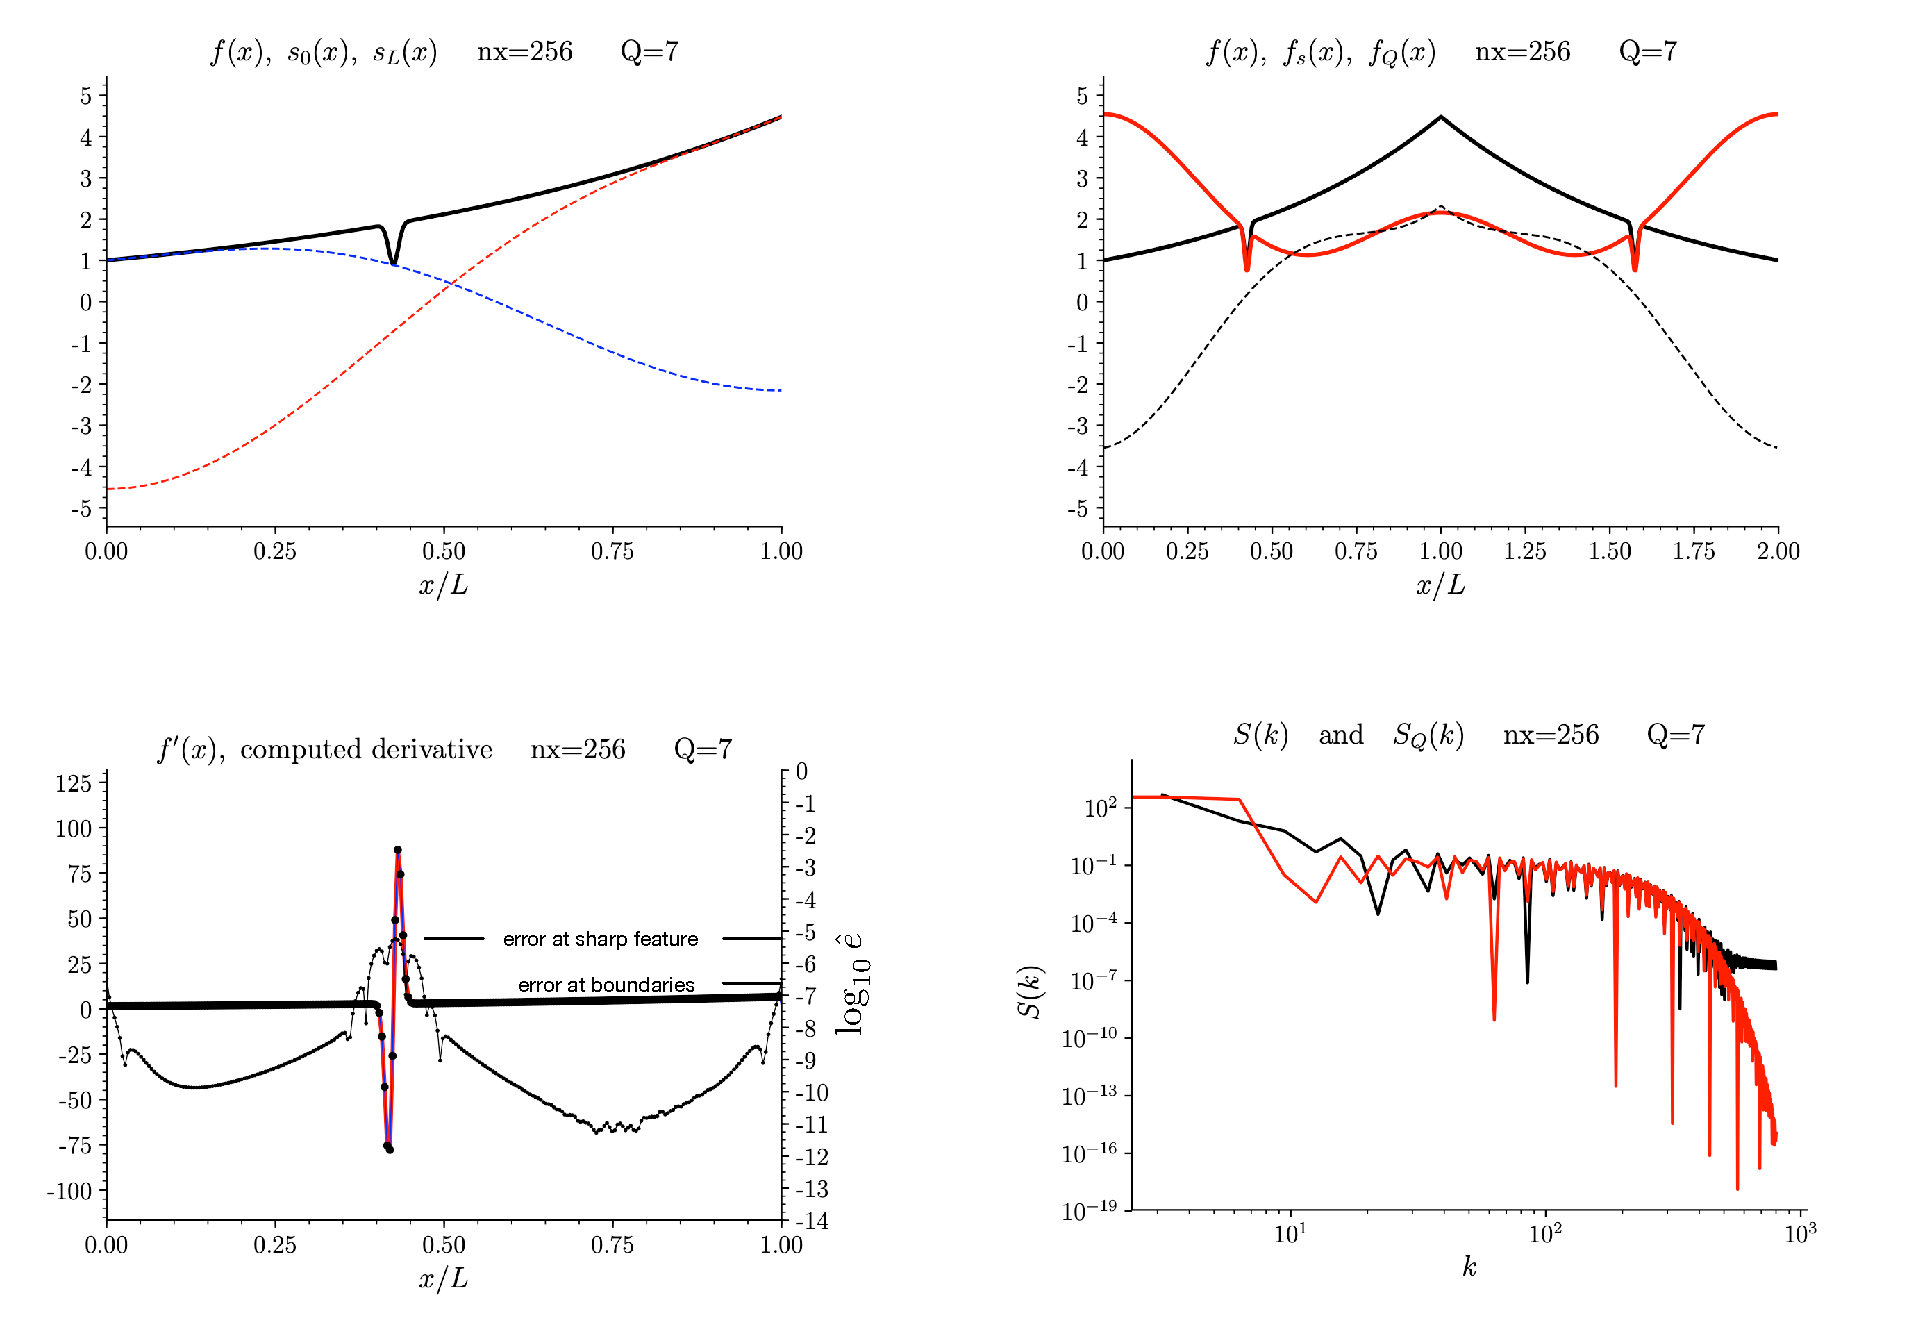
\includegraphics[width=1.0\textwidth]{FIGS/trig_figs/bump.eps}}
  \caption{Example function that varies at large scale across the domain but has a sharp feature in the interior. Quantities shown in the figure are as in the previous figures.}
   \label{fig:bump}
\end{figure}


\bibliographystyle{jfm}
% Note the spaces between the initials
\bibliography{ttbl.bib}

\end{document}
